% Shared preamble for the Radioactive Signal Explorer explainers (docs/signals/*.tex).
\documentclass[11pt]{article}
\usepackage[letterpaper,margin=1in]{geometry}
\usepackage[T1]{fontenc}
\usepackage{lmodern}
\usepackage{microtype}
\usepackage{amsmath,amssymb,mathtools,bm}
\usepackage{siunitx}
\usepackage{graphicx}
\usepackage{booktabs,array,tabularx}
\usepackage{xcolor}
\usepackage{enumitem}
\usepackage{caption}
\usepackage[section]{placeins}
\usepackage[most]{tcolorbox}
\usepackage[colorlinks=true,linkcolor=blue!50!black,citecolor=blue!50!black,urlcolor=blue!50!black]{hyperref}
\usepackage[capitalise,noabbrev]{cleveref}
\sisetup{group-separator={,},group-minimum-digits=4,separate-uncertainty}
\definecolor{labblue}{HTML}{0088EE}
\definecolor{exbg}{HTML}{FFF7EC}
\definecolor{boxbg}{HTML}{EEF4FB}
\newtcolorbox{keyidea}[1][]{colback=boxbg,colframe=labblue,boxrule=0.6pt,arc=2pt,left=6pt,right=6pt,top=4pt,bottom=4pt,fonttitle=\bfseries,title={#1}}
\newtcolorbox{pitfall}[1][]{colback=red!3,colframe=red!55!black,boxrule=0.6pt,arc=2pt,left=6pt,right=6pt,top=4pt,bottom=4pt,fonttitle=\bfseries,title={#1}}
\newcounter{exercise}
\newtcolorbox{exercise}[1][]{colback=exbg,colframe=orange!70!black,boxrule=0.6pt,arc=2pt,left=6pt,right=6pt,top=4pt,bottom=4pt,fonttitle=\bfseries,
  title={Exercise~\refstepcounter{exercise}\theexercise\ifx\relax#1\relax\else\ (#1)\fi}}
\newcommand{\dd}{\mathrm{d}}
\newcommand{\keV}{\,\mathrm{keV}}
\newcommand{\MeV}{\,\mathrm{MeV}}
\newcommand{\me}{m_e c^2}
\newcommand{\nuc}[2]{${}^{#1}$#2}
\newcommand{\code}[1]{\texttt{#1}}
\newcommand{\explorer}{\href{https://dark-matter.ucr.edu/Signals.html}{Radioactive Signal Explorer}}
\newcommand{\seriesnote}{\noindent\small This note is one of five explaining the physics behind the \explorer: gamma rays, alpha decay, $(\alpha,n)$ neutrons, beta decay and Cherenkov light. Every figure was computed with the page's own code (\code{assets/signals-physics.js}); the \LaTeX{} sources and figure scripts are in \code{docs/signals/} of \url{https://github.com/UCRDarkMatter/dark-matter-lab-site}. Exercises are marked (A) analytic, (P) programming, (R) open-ended.\normalsize}

\title{Gamma Rays in a Detector:\\ Cross Sections, Compton Continua and Escape Peaks}
\author{UCR Dark Matter Lab --- notes for graduate students}
\date{\today}
\begin{document}
\maketitle
\seriesnote

\begin{abstract}
A gamma ray of energy $E_\gamma$ does not deposit $E_\gamma$ in a detector. It deposits whatever its first interaction, and the fate of the secondaries, leave behind: a Compton continuum ending at an edge, a full-energy peak, X-ray escape peaks, and single- and double-escape peaks. This note derives each piece from the interaction cross sections, explains how the Gamma tab of the Signal Explorer builds a deposited-energy spectrum from NIST XCOM data, and shows where that one-interaction model stops being adequate.
\end{abstract}
\tableofcontents

\section{Photon interactions}
Between roughly \SI{10}{keV} and \SI{10}{MeV} four processes matter:
\begin{description}[leftmargin=1.5em]
\item[Photoelectric absorption] The photon is absorbed by a bound electron, which leaves with $T = E_\gamma - B_i$ (shell binding energy $B_i$). It dominates at low energy and high $Z$, scaling roughly as $Z^{4\text{--}5}/E_\gamma^{3}$, with sawtooth edges where a new shell becomes accessible.
\item[Incoherent (Compton) scattering] The photon scatters off an (effectively free) electron and survives at lower energy. Per electron, so per gram it scales as $Z/A \approx 1/2$ for everything but hydrogen.
\item[Pair production] Above $2\me = \SI{1022}{keV}$ the photon converts to $e^+e^-$ in the field of a nucleus ($\propto Z^2$); above $4\me$ also in the field of an atomic electron (triplet production, $\propto Z$).
\item[Coherent (Rayleigh) scattering] Elastic scattering off the whole atom. It changes the direction but deposits nothing, so it is irrelevant to the spectrum (it only matters for attenuation and imaging).
\end{description}

The mass attenuation coefficient of a compound or mixture with mass fractions $w_j$ is additive:
\begin{equation}
\frac{\mu}{\rho}(E) = \sum_j w_j \left(\frac{\mu}{\rho}\right)_j(E), \qquad \left(\frac{\mu}{\rho}\right)_j = \frac{N_A}{A_j}\,\sigma_j(E),
\label{eq:mix}
\end{equation}
and the probability that a photon's first non-coherent interaction is of type $k$ is
\begin{equation}
f_k = \frac{\mu_k}{\mu_\text{photo} + \mu_\text{incoh} + \mu_\text{pair}}.
\label{eq:fk}
\end{equation}
The explorer takes $\mu_k/\rho$ per element from NIST XCOM \cite{xcom} (fetched by a GitHub workflow into \code{data/signals/xcom.json}) and interpolates log--log, which is accurate between tabulated points everywhere except across an absorption edge (XCOM lists the energy twice at an edge, once on each side). \Cref{fig:xcom} shows the result for three common detector media.

\begin{figure}[htbp]
\centering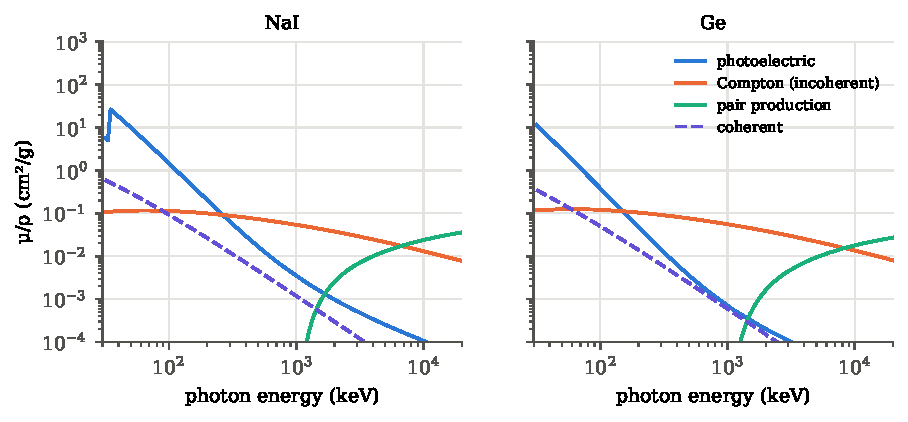
\includegraphics[width=\linewidth]{fig/g_xcom.pdf}
\caption{Partial mass attenuation coefficients from XCOM for NaI, germanium and water. Note the K edges of iodine (\SI{33.2}{keV}) and germanium (\SI{11.1}{keV}, off scale), the near-universal Compton curve (per gram it depends only on $Z/A$; water is higher because of hydrogen), and pair production overtaking Compton above \SIrange{5}{10}{MeV}.}
\label{fig:xcom}
\end{figure}

\begin{keyidea}[Attenuation length vs.\ interaction mix]
The \emph{attenuation length} $1/\mu$ decides whether the photon interacts at all; the \emph{fractions} $f_k$ decide what the first interaction is. A \SI{662}{keV} photon in NaI has $1/\mu \approx \SI{3.6}{cm}$, and its first interaction is Compton scattering 88\% of the time. A full-energy peak nevertheless exists because the scattered photon can be absorbed later: that is what the escape probability below parametrises.
\end{keyidea}

\section{Compton scattering}
\subsection{Kinematics}
For a photon of energy $E$ scattering through angle $\theta$ off an electron at rest, energy--momentum conservation gives
\begin{equation}
E' = \frac{E}{1 + \varepsilon(1-\cos\theta)}, \qquad \varepsilon \equiv \frac{E}{\me},
\label{eq:compton}
\end{equation}
so the electron receives $T = E - E'$. The maximum, at $\theta = \pi$, is the \emph{Compton edge},
\begin{equation}
T_\text{max} = E\,\frac{2\varepsilon}{1+2\varepsilon},
\label{eq:edge}
\end{equation}
and the corresponding back-scattered photon has $E'_\text{min} = E/(1+2\varepsilon)$, which approaches $\me/2 = \SI{255.5}{keV}$ for large $E$. Photons that back-scatter from material \emph{around} the detector and are then absorbed produce the familiar back-scatter peak at $E'_\text{min}$ (\SI{184}{keV} for \nuc{137}{Cs}).

\subsection{Klein--Nishina}
The differential cross section per electron, to lowest order in QED, is the Klein--Nishina formula. Changing variables from $\cos\theta$ to $s = T/E$ using $\dd T/\dd\cos\theta = E'^2/\me$ gives
\begin{equation}
\frac{\dd\sigma}{\dd T} = \frac{\pi r_e^2}{\me\,\varepsilon^2}
\left[\,2 + \frac{s^2}{\varepsilon^2(1-s)^2} + \frac{s}{1-s}\left(s - \frac{2}{\varepsilon}\right)\right],
\qquad 0 \le s \le \frac{2\varepsilon}{1+2\varepsilon},
\label{eq:kn}
\end{equation}
which is what \code{knShape(E, T)} evaluates (without the prefactor, then normalised numerically). Its integral is the KN total cross section
\begin{equation}
\sigma_\text{KN} = 2\pi r_e^2\left\{\frac{1+\varepsilon}{\varepsilon^2}\left[\frac{2(1+\varepsilon)}{1+2\varepsilon} - \frac{\ln(1+2\varepsilon)}{\varepsilon}\right] + \frac{\ln(1+2\varepsilon)}{2\varepsilon} - \frac{1+3\varepsilon}{(1+2\varepsilon)^2}\right\}.
\end{equation}
The shape (\cref{fig:kn}) is flat-ish at low energy and develops a pronounced pile-up just below the edge at high energy, because $\dd T/\dd\cos\theta$ vanishes at $\theta=\pi$.

\begin{figure}[htbp]
\centering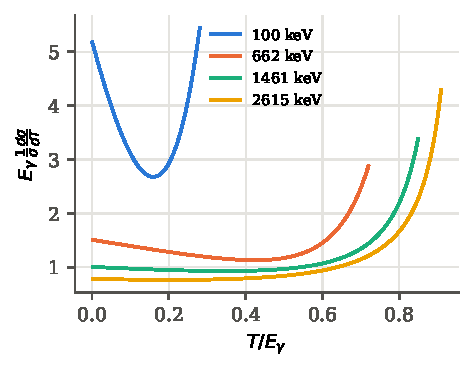
\includegraphics[width=0.62\linewidth]{fig/g_kn.pdf}
\caption{Klein--Nishina recoil-electron spectra, normalised to unit area and plotted against $T/E_\gamma$. The edge moves towards $T/E_\gamma = 1$ as $\varepsilon$ grows.}
\label{fig:kn}
\end{figure}

\begin{pitfall}[What Klein--Nishina leaves out]
\Cref{eq:kn} assumes free electrons at rest. Binding (the incoherent scattering function $S(x,Z)$) suppresses small-angle, low-$T$ scattering, and electron motion (Doppler broadening) rounds the Compton edge by a few keV in high-$Z$ material. XCOM's \emph{total} incoherent cross section includes binding; the explorer's \emph{shape} does not. For a scintillator the energy resolution hides both; for HPGe the rounded edge is visible.
\end{pitfall}

\section{Building a deposited-energy spectrum}
\subsection{The one-interaction model}
The explorer follows the first interaction exactly and treats everything after it with one number, the probability $p_\text{esc}$ that a \emph{secondary photon} (scattered photon, fluorescence X-ray or annihilation photon) leaves the detector without depositing anything. $p_\text{esc}=1$ is the thin-detector limit; $p_\text{esc}=0$ is an infinite detector, where every photon ends in the full-energy peak. The deposited-energy density per interacting photon is then
\begin{align}
\frac{\dd N}{\dd E_\text{dep}} =\;&
f_C\,p_\text{esc}\,\frac{1}{\sigma}\frac{\dd\sigma}{\dd T}\Big|_{T=E_\text{dep}}
\nonumber\\
&+ \Big[f_P(1-x_K) + f_C(1-p_\text{esc}) + f_X(1-p_\text{esc})^2\Big]\,\delta(E_\text{dep} - E)
\;+\; f_P\,x_K\,\delta(E_\text{dep} - E + E_{K\alpha})\nonumber\\
&+ f_X\Big[2p_\text{esc}(1-p_\text{esc})\,\delta(E_\text{dep} - E + \me) + p_\text{esc}^2\,\delta(E_\text{dep} - E + 2\me)\Big],
\label{eq:model}
\end{align}
with $f_C, f_P, f_X$ from \cref{eq:fk} and the X-ray escape probability $x_K$ defined below. Each delta function is then convolved with a Gaussian of width
\begin{equation}
\sigma(E) = \frac{\text{FWHM}_{662}}{2.3548}\sqrt{\frac{E}{\SI{662}{keV}}},
\label{eq:res}
\end{equation}
the Poisson-statistics scaling appropriate for a scintillator; for a semiconductor a constant term should be added in quadrature.

The middle term of \cref{eq:model} is worth pausing on: a Compton-scattered photon that is subsequently absorbed puts the \emph{full} energy in the detector, so Compton scattering feeds the full-energy peak. In a large detector most of the photopeak comes from multiple Compton scatters, not from single photoabsorption. \Cref{fig:cs} shows the three regimes for \nuc{137}{Cs} in NaI.

\begin{figure}[htbp]
\centering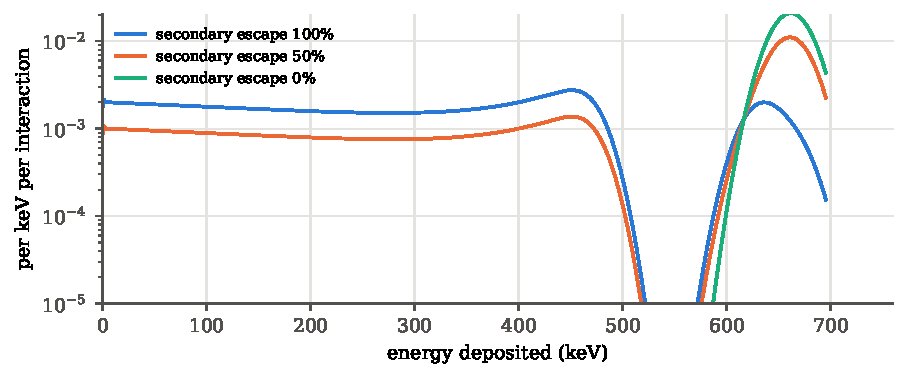
\includegraphics[width=0.66\linewidth]{fig/g_cs.pdf}
\caption{Deposited energy per interacting \SI{661.7}{keV} photon in NaI with $\text{FWHM}_{662} = \SI{45}{keV}$, for three values of the secondary escape probability. The Compton continuum shrinks and the full-energy peak grows as the detector gets larger. The iodine K X-ray escape peak (\SI{\approx 29}{keV} below the photopeak) is hidden in the photopeak at this resolution.}
\label{fig:cs}
\end{figure}

\begin{keyidea}[Why ``probability of escape'' is a crude but useful knob]
In reality $p_\text{esc}$ depends on where the first interaction happened, on the secondary's energy and direction, and on the detector geometry. A single number cannot reproduce, e.g., the multiple-Compton events that fill the valley between the Compton edge and the photopeak. That is a job for Geant4. What the one-number model gets right is \emph{where} every feature is and roughly \emph{how big} it is, which is what you need to identify a line or to sanity-check a simulation.
\end{keyidea}

\subsection{Photoabsorption and X-ray escape}
After photoabsorption on the K shell the atom relaxes by emitting either a K X-ray (probability $\omega_K$, the fluorescence yield) or an Auger electron. If the X-ray escapes, the deposited energy is $E - E_{K\alpha}$. The explorer
\begin{itemize}
\item picks the element with the largest photoelectric contribution (the ``dominant absorber'');
\item assumes 80\% of photoabsorptions above the K edge are on the K shell (the K-shell jump ratio gives 0.8--0.9 for medium and high $Z$);
\item uses the Bambynek fit for the fluorescence yield \cite{bambynek},
\begin{equation}
\omega_K = \frac{a^4}{1+a^4}, \qquad a = 0.015 + 0.0327\,Z - 0.64\times10^{-6}\,Z^3;
\end{equation}
\item and a Moseley-law estimate $E_{K\alpha} \approx 10.2\,\mathrm{eV}\,(Z-1)^2$ with a small relativistic correction, capped at the K edge taken from XCOM.
\end{itemize}
Then $x_K = 0.8\,\omega_K\,p_\text{esc}$. For iodine $\omega_K = 0.88$ and $E_{K\alpha} \approx \SI{29.6}{keV}$ (measured \SI{28.6}{keV}; the Moseley estimate is good to a few per cent); for germanium $\omega_K = 0.54$ and $E_{K\alpha} \approx \SI{10.1}{keV}$ (measured \SI{9.9}{keV}). These are the escape peaks that appear just below low-energy lines in HPGe spectra.

\subsection{Pair production and escape peaks}
After pair production the $e^+$ and $e^-$ share $E - 2\me$ and deposit it locally; the positron then annihilates (almost always at rest) into two back-to-back \SI{511}{keV} photons. With independent escape probabilities for the two photons, the deposited energy is
\begin{equation}
E_\text{dep} = \begin{cases} E - 2\me & \text{probability } p_\text{esc}^2 \text{ (double escape)}\\
E - \me & 2p_\text{esc}(1-p_\text{esc}) \text{ (single escape)}\\
E & (1-p_\text{esc})^2 \text{ (full energy)}\end{cases}
\end{equation}
(treating partial deposition by a Compton-scattered annihilation photon as either escape or full absorption, the same approximation as above).

The energy sharing between $e^+$ and $e^-$ matters for anything that depends on individual particle energies---for example the Cherenkov light they emit. The explorer uses the unscreened Bethe--Heitler distribution in the Born approximation \cite{bethe-heitler,motz}: with $W_\pm$ the total energies in units of $\me$ and $k = E/\me$,
\begin{equation}
\frac{\dd\sigma}{\dd W_+} \propto \frac{1}{k^3}\left(W_+^2 + W_-^2 + \tfrac{2}{3}W_+W_-\right)\left(\ln\frac{2W_+W_-}{k} - \tfrac12\right),
\qquad W_+ + W_- = k,
\label{eq:bh}
\end{equation}
which is symmetric and fairly flat except near the ends (\cref{fig:pair}). Close to threshold the logarithm becomes negative and the Born approximation fails; there the code falls back to the phase-space shape $p_+p_-W_+W_-$. Coulomb corrections make the real distribution slightly asymmetric (the positron is pushed to higher energy by the nucleus), an effect of a few per cent at these energies that \cref{eq:bh} does not include.

\begin{figure}[htbp]
\centering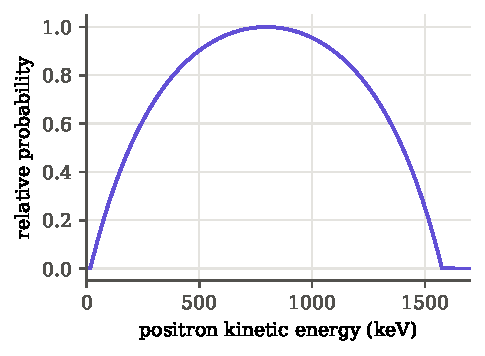
\includegraphics[width=0.6\linewidth]{fig/g_pair.pdf}
\caption{Bethe--Heitler positron kinetic-energy distribution for the \SI{2614.5}{keV} line of \nuc{208}{Tl} in germanium. The positron and electron share $E-2\me = \SI{1592}{keV}$.}
\label{fig:pair}
\end{figure}


\section{Beyond the gamma: conversion, pairs and cascades}
\subsection{Internal conversion, X-rays and Auger electrons}
A nuclear transition can give its energy to an atomic electron instead of emitting a photon. The total conversion coefficient $\alpha = N_e/N_\gamma$ (tabulated by BrIcc \cite{bricc} and carried in ENSDF) grows steeply with multipolarity and $Z$ and falls with energy. Per decay, a line with photon intensity $I_\gamma$ is accompanied by $I_\gamma\alpha$ conversion electrons of energy $E_\gamma - B_i$, with $B_i$ the binding energy of the shell ($K$, $L$, \dots). The vacancy then fills by X-ray emission (fluorescence yield $\omega_K$) or Auger electrons. The tab lists the ENSDF electron lines when they exist; otherwise it estimates them from $\alpha$, placing all of them at $E_\gamma - B_K$. In a source embedded in a calorimeter the electron, X-ray and Auger energies are all absorbed, so the full transition energy is seen even though no gamma left the nucleus.

\subsection{Internal pair creation}
Above $2\me$ the nucleus can create an $e^+e^-$ pair directly. In the Born approximation (Rose; Goldring \cite{goldring}) the differential coefficient for an electric (E1) or magnetic (M1) dipole of energy $k$ (in units of $\me$) is
\begin{equation}
\frac{\dd\alpha_\pi}{\dd E_+\,\dd\Omega_+\,\dd\Omega_-} = \frac{\alpha}{16\pi^3}\frac{p_+p_-}{k^3}\left[\frac{4k^2}{(k^2-q^2)^2} + \frac{2(p_+^2+p_-^2)}{k^2-q^2} \pm 1\right],
\end{equation}
with $q = |\vec p_+ + \vec p_-|$, $+$ for E1 and $-$ for M1. Integrated it gives $\alpha_\pi \sim 10^{-4}$--$10^{-3}$ (e.g.\ $3.2\times10^{-3}$ for an \SI{18.15}{MeV} M1, the \nuc{8}{Be} transition behind the ATOMKI ``X17'' anomaly \cite{atomki}). The pair deposits $E - 2\me$ locally and two \SI{511}{keV} photons follow. The opening-angle distribution peaks at small angles and falls monotonically; a light boson decaying to $e^+e^-$ would instead give a bump at $\cos\theta \approx 1 - 2m_X^2/E^2$.

\subsection{Cascades: coincidence summing and angular correlations}
When a level decays through intermediate states, the gammas are emitted within picoseconds and a detector sees them together. If both interact, their deposits add (true coincidence summing): counts move out of the single-line peaks and into sum peaks such as \SI{2505.7}{keV} for \nuc{60}{Co}. The tab's Monte Carlo builds the cascades from the level scheme. The net feeding of each level is the intensity leaving it minus the intensity arriving. Each branch is chosen with probability $\propto I_\gamma(1+\alpha)$, and a branch is a photon with probability $1/(1+\alpha)$ and a conversion electron otherwise. The directions of successive gammas are correlated:
\begin{equation}
W(\theta) = 1 + A_{22}P_2(\cos\theta) + A_{44}P_4(\cos\theta),\qquad A_{kk} = A_k(\gamma_1)A_k(\gamma_2),
\end{equation}
with $A_k$ built from the $F_k(L,L',J_i,J)$ coefficients and the mixing ratios $\delta$ \cite{krane}. For \nuc{60}{Co} ($4^+\to2^+\to0^+$, E2--E2) $A_{22} = 0.102$ and $A_{44} = 0.009$. Close geometries enhance the effect because the second photon prefers to go along or against the first.

\subsection{Doppler broadening}
A gamma emitted by a recoiling nucleus is shifted by $E_\gamma\beta\cos\theta$. For isotropic emission at constant speed this gives a flat box of half-width $E_\gamma\beta$. If the emitter slows down over a time comparable to the level's mean life $\tau$, the box shrinks as it decays, and a fraction $e^{-t_\text{stop}/\tau}$ is emitted at rest as a narrow line. The \SI{478}{keV} line from \nuc{10}{B}$(n,\alpha)$\nuc{7}{Li}$^*$ (\nuc{7}{Li} recoiling with \SI{840}{keV}, $\tau \approx \SI{105}{fs}$) is about \SI{15}{keV} wide, which matters when using boron-loaded scintillators for neutron tagging.

\subsection{A small photon Monte Carlo}
The single-knob model of \cref{eq:model} is replaced in the Monte Carlo by actual tracking in a sphere or cylinder. Interaction points are sampled from $\mu(E)$. Compton scattering is sampled from Klein--Nishina (Kahn's method). Photoabsorption may emit a $K$ X-ray, which is tracked. Pair production deposits $E - 2\me$ and tracks two back-to-back annihilation photons. Electrons deposit locally. The source can sit at the centre, be spread through the volume, or sit on the axis outside.
\section{What the Gamma tab outputs}
For an energy, or for every line of a chosen isotope weighted by its intensity, the tab shows the components of \cref{eq:model} on a common grid and lists the discrete features (full-energy peak, X-ray escape, single and double escape, Compton edge, back-scatter energy) with their weights. The CSV contains the same columns. The ``electrons'' spectrum passed to the Cherenkov tab is different: it is the kinetic energy given to \emph{electrons} by the first interaction (KN recoils, photoelectrons at $E - B_K$, and both pair leptons), because that is what radiates.

\section{Exercises}
\begin{exercise}[A]
Derive \cref{eq:compton} from four-momentum conservation. Show that $T_\text{max} \to E - \me/2$ for $E \gg \me$.
\end{exercise}
\begin{exercise}[A]
Starting from the Klein--Nishina formula in the form $\dd\sigma/\dd\Omega = \tfrac{r_e^2}{2}(E'/E)^2\left(E'/E + E/E' - \sin^2\theta\right)$, change variables to $T$ and recover \cref{eq:kn}.
\end{exercise}
\begin{exercise}[A]
Using \cref{eq:model} with $p_\text{esc}$ as a free parameter, write the peak-to-total ratio as a function of $f_C$, $f_P$, $f_X$ and $p_\text{esc}$. For \nuc{137}{Cs} in NaI ($f_P \approx 0.12$, $f_C \approx 0.88$ from XCOM), what $p_\text{esc}$ gives the peak-to-total of about 0.3 typical of a \SI{3}{in}$\times$\SI{3}{in} crystal? Comment on why the result is smaller than the geometric escape probability you might estimate from the attenuation length of a \SI{480}{keV} photon.
\end{exercise}
\begin{exercise}[P]
Implement \cref{eq:mix,eq:fk} for a mixture using the XCOM tables in \code{data/signals/xcom.json}. Plot $f_P$, $f_C$, $f_X$ versus energy for liquid argon and for xenon, and find the energy at which Compton scattering overtakes photoabsorption in each.
\end{exercise}
\begin{exercise}[P]
Write a toy Monte Carlo for a sphere of NaI of radius $R$ with a \SI{662}{keV} source at the centre: sample the first interaction point and type, KN-sample the scattered photon direction, and track it until it escapes or is absorbed (repeat for multiple scatters). Compare the spectrum with \cref{eq:model} and determine the effective $p_\text{esc}(R)$ that best reproduces your peak-to-total.
\end{exercise}
\begin{exercise}[R]
In an HPGe spectrum of a thorium source you see a peak at \SI{1592}{keV}, one at \SI{2103}{keV}, and one at \SI{511}{keV}. Explain each, and explain why the \SI{511}{keV} peak is broader than neighbouring lines.
\end{exercise}

\begin{thebibliography}{9}
\bibitem{xcom} M.~J. Berger \emph{et al.}, \emph{XCOM: Photon Cross Sections Database}, NIST Standard Reference Database 8, \url{https://www.nist.gov/pml/xcom-photon-cross-sections-database}.
\bibitem{bambynek} W.~Bambynek \emph{et al.}, ``X-ray fluorescence yields, Auger, and Coster--Kronig transition probabilities'', Rev.\ Mod.\ Phys.\ \textbf{44}, 716 (1972).
\bibitem{bethe-heitler} H.~Bethe and W.~Heitler, ``On the stopping of fast particles and on the creation of positive electrons'', Proc.\ R.\ Soc.\ A \textbf{146}, 83 (1934).
\bibitem{motz} J.~W. Motz, H.~A. Olsen and H.~W. Koch, ``Pair production by photons'', Rev.\ Mod.\ Phys.\ \textbf{41}, 581 (1969).
\bibitem{knoll} G.~F. Knoll, \emph{Radiation Detection and Measurement}, 4th ed.\ (Wiley, 2010), ch.~2 and 10.
\bibitem{bricc} T.~Kib\'edi \emph{et al.}, ``Evaluation of theoretical conversion coefficients using BrIcc'', Nucl.\ Instrum.\ Meth.\ A \textbf{589}, 202 (2008).
\bibitem{goldring} G.~Goldring, ``Internal pair formation'', Proc.\ Phys.\ Soc.\ A \textbf{66}, 341 (1953); M.~E. Rose, Phys.\ Rev.\ \textbf{76}, 678 (1949).
\bibitem{atomki} A.~J. Krasznahorkay \emph{et al.}, Phys.\ Rev.\ Lett.\ \textbf{116}, 042501 (2016).
\bibitem{krane} K.~S. Krane, R.~M. Steffen and R.~M. Wheeler, ``Directional correlations of gamma radiations emitted from nuclear states'', Nucl.\ Data Tables \textbf{11}, 351 (1973).
\end{thebibliography}
\end{document}
